%==========================================================
% This is for generating a standalone project requirements
%==========================================================
\documentclass[a4paper, 11pt]{report}
\usepackage[T1]{fontenc}
\usepackage[utf8]{inputenc}
\usepackage[english]{babel}
\usepackage{graphicx} % support graphics
\usepackage{hyperref} % links in the document
\usepackage{float} % position of figures
\usepackage{paralist} % inline lists
\usepackage{verbatim} % multiline comments
\usepackage[table]{xcolor} % table row coloring
\usepackage{booktabs} % Professional tables
\usepackage{tabularx} % Simple column stretching
\usepackage{multirow} % Row spanning
\usepackage{wrapfig} % Wrap text around figures
\usepackage{array} 
\usepackage{longtable}
\usepackage{listings}
\usepackage{color}
\usepackage{textcomp}
\usepackage[style=treenoname,subentrycounter,numberedsection, 
        section=chapter, acronym]{glossaries}


% Configure links in pdfs
\hypersetup{
    bookmarksopen=false, % Hide bookmarks menu
    colorlinks=true, % Don't wrap links in colored boxes
}

\title{Project Requirements}
\author{Kpro group 9}
\date{\today}

\begin{document}
%\maketitle
%\tableofcontents
\makeglossaries
\newglossaryentry{wireshark}{name={Wireshark},
description={Program used to analyze packet data sent between network nodes}}

\newglossaryentry{python}{name={Python},
description={A programming language}}

\newglossaryentry{mac}{name={Mac},
description={A brand of personal computers}}

\newglossaryentry{linux}{name={Linux},
description={An operating system}}

\newglossaryentry{c}{name={C},
description={A programming language}}

\newglossaryentry{clang}{name={clang},
description={A compiler front-end for different \Gls{c} programming languages}}

\newglossaryentry{gcc}{name={gcc},
description={define this}}

\newglossaryentry{c++}{name={C++},
description={A programming language}}

\newglossaryentry{java}{name={Java},
description={A programming language}}

\newglossaryentry{lua}{name={Lua},
description={A programming language, often used for making \glspl{script}}}

\newglossaryentry{script}{name={script},
description = {A list of commands that are executed by a certain program, usually as an extension of the original functionality},
plural=scripts} 

\newglossaryentry{int}{name={int},
description={See \gls{integer}}}

\newglossaryentry{double}{name={double},
description={DEFINE}}

\newglossaryentry{integer}{name={integer},
description={define this},
plural=integers}

\newglossaryentry{char}{name={char},
description={define this},
plural=chars}

\newglossaryentry{float}{name={float},
description={define this},
plural=floats}

\newglossaryentry{pycparser}{name={pycparser},
description={A \Gls{c} \gls{parser} written in \Gls{python}}}

\newglossaryentry{ply}{name={ply},
description = {A \Gls{python} \gls{library} for creating \glspl{lexer} and \glspl{parser}}}

\newglossaryentry{parser}{name={parser},
description = {A program that receives input, checks it for correct syntax and builds a data structure representing the input},
plural=parsers}

\newglossaryentry{lexer}{name={lexer},
description = {A lexer is a program that converts a sequence of characters into a sequence of tokens},
plural=lexers}

\newglossaryentry{token}{name={token},
description = {A string of characters, categorized as a symbol according to a set of given rules},
plural=tokens}

\newglossaryentry{dissector}{name={dissector},
description = {Code that decodes \gls{packet} data and makes it readable by humans},
plural=dissectors}

\newglossaryentry{packet}{name={packet},
description = {Small block of data transmitted over a network},
plural=packets}

\newglossaryentry{utility}{name={utility},
description = {A small program that supports larger applications by doing certain tasks},
plural=utilities}

\newglossaryentry{library}{name={library},
description = {A collection of pre-written code for aiding programmers in the development process},
plural=libraries}

\newglossaryentry{ipc}{name={inter-process communication},
description = {The exchange of data that happens between \glspl{process}}}

\newglossaryentry{process}{name={process},
description = {A program running on a computer},
plural=processes}

\newglossaryentry{struct}{name={struct},
description = {Short for structure, it is a type that groups several \glspl{member} into a single \gls{object}},
plural=structs}

\newglossaryentry{member}{name={member},
description = {define this},
plural=members}

\newglossaryentry{binary}{name={binary},
description = {Two base arithmetic using the digits 0 and 1}}

\newglossaryentry{binary file}{name={binary file},
description = {A computer-readable file stored in \gls{binary} format}}

\newglossaryentry{nested struct}{name={nested struct},
description = {A \gls{struct} within another \gls{struct}},
plural={nested structs}}

\newglossaryentry{sparc}{name={SPARC},
description={A microprocessor architecture based on reduced instruction set computing}}

\newglossaryentry{version control system}{name={version control system},
description = {A system that ensures consistency of files when several people are collaborating on them},
plural={version control systems}}

\newglossaryentry{scrum}{name={Scrum},
description={A \gls{software development methodology}}}

\newglossaryentry{software development methodology}{name={software development methodology},
description={A framework used to structure, plan and control a development process},
plural={software development methodologies}}

\newglossaryentry{branch}{name={branch},
description={define this},
plural=branches}

\newglossaryentry{distributed repository model}{name={distributed repository model},
description={A distributed approach to a \gls{version control system}},
plural={distributed repository models}}

\newglossaryentry{markup language}{name={markup language},
description={A language for specifying the processing, definition and presentation of text}}

\newglossaryentry{capture file}{name={capture file},
description={A file containing the data that is captured from network or IPC traffic},
plural={capture files}}

\newglossaryentry{ascii}{name={ASCII},
description={A character encoding scheme}}

\newglossaryentry{character encoding scheme}{name={character encoding scheme},
description={A system that maps characters to something else, write more }}

\newglossaryentry{hexadecimal}{name={hexadecimal},
description={A number system where sixteen is the base}}

\newglossaryentry{hex dump}{name={hex dump},
description={A \gls{hexadecimal} view of computer data},
plural={hex dumps}}

\newglossaryentry{pcap-file}{name={pcap-file},
description={See \gls{capture file}},
plural={pcap-files}}

\newglossaryentry{protocol}{name={protocol},
description = {A system of rules for exchanging messages between machines},
plural=protocols}

\newglossaryentry{link-layer}{name={link-layer},
description = {The \gls{protocol} layer that is responsible for transferring data between two nodes}}

\newglossaryentry{repository}{name={repository},
description = {A central storage area where data is kept and maintained},
plural=repositories}

\newglossaryentry{Sun RPC}{name={Sun RPC},
description={The Unix equivalent of Remote Procedure Call}}

\newglossaryentry{corba}{name={CORBA},
description={This is an acronym}}

\newglossaryentry{asn1}{name={ASN.1},
description={This is an acronym}}

\newglossaryentry{makefile}{name={makefile},
description={A file that helps the make utility in the creation of executables from source code},
plural=makefiles}

\newglossaryentry{post-dissector}{name={post-dissector},
description = {define this},
plural=post-dissectors}

\newglossaryentry{boolean}{name={boolean},
description={A data type that represents logical truth, it has the value True or False},
plural=booleans}

\newglossaryentry{string}{name={string},
description={define this},
plural=strings}

\newglossaryentry{garbage collection}{name={garbage collection},
description={define this}}

\newglossaryentry{closure}{name={closure},
description={define this},
plural=closures}

\newglossaryentry{object}{name={object},
description = {define this},
plural=objects}

\newglossaryentry{C99}{name={C99},
description={define this}}

\newglossaryentry{GCC-XML}{name={GCC-XML},
description={define this}}

\newglossaryentry{xml}{name={xml},
description={A \gls{markup language}}}

\newglossaryentry{Objective-C++}{name={Objective-C++},
description={A programming language}}

\newglossaryentry{Objective-C}{name={Objective-C},
description={A programming language}}

\newglossaryentry{AST}{name={abstract syntax tree},
description={A tree represention of a compiled program}}

\newglossaryentry{data serialization}{name={data serialization},
description={define this}}

\newglossaryentry{perl}{name={perl},
description={A programming language}}

\newglossaryentry{php}{name={php},
description={A scripting language}}

\newglossaryentry{Ruby}{name={Ruby},
description={A programming language}}

\newglossaryentry{Javascript}{name={Javascript},
description={A scripting language}}

\newglossaryentry{Eclipse}{name={Eclipse},
description={An application aiding computer programmers in software development}}

\newglossaryentry{header}{name={header},
description={define this},
plural=headers}

\newglossaryentry{enumerated named value}{name={enumerated named value},
description={define this},
plural={enumerated named values}}

\newglossaryentry{union}{name={union},
description={define this},
plural=unions}

\newglossaryentry{array}{name={array},
description={A data type that can hold a collection of elements},
plural=arrays}

\newglossaryentry{preprocessor}{name={preprocessor},
description={Define this},
plural=preprocessors}

\newglossaryentry{include}{name={\#include},
description={A \Gls{c} directive that includes other \gls{header} files to the current file}}

\newglossaryentry{if}{name={\#if},
description={A \Gls{c} directive that executes a statement if a given expression holds true }}

\newglossaryentry{ifdef}{name={\#ifdef},
description={A \Gls{c} directive that checks if a given token has been defined}}

\newglossaryentry{define}{name={\#define},
description={A \Gls{c} directive that can be used to define a constant or create a macro}}

\newglossaryentry{trailers}{name={trailers},
description={define this}}

\newglossaryentry{bit string}{name={bit string},
description={define this}
plural={bit strings}}

\newglossaryentry{endian}{name={endian},
description={See \gls{endianness}},
plural=endians}

\newglossaryentry{endianness}{name={endianness},
description={Refers to the ordering of bytes in a word. A big-endian machine stores the most significant byte first, and a little-endian the least significant.}}

\newglossaryentry{batch mode}{name={batch mode},
description={define this}}

\newglossaryentry{batch processing}{name={batch processing},
description={See \gls{batch mode}}}

\newglossaryentry{x86}{name={x86},
description={The instruction set architecture used by Intel processors}}

\newglossaryentry{Windows}{name={Windows},
description={An operating system by Microsoft}}

\newglossaryentry{Solaris}{name={Solaris},
description={An operating system by Sun Microsystems}}

\newglossaryentry{x86-64}{name={x86-64},
description={An extension of the \gls{x86} instruction set that is compatible with 64-bit processors}}

\newglossaryentry{Field}{name={Field},
description={define this}}

\newglossaryentry{argparse}{name={argparse},
description={define this}}

\newglossaryentry{enum}{name={enum},
description={See /gls{enumerated named value}},
plural=enums}

\newglossaryentry{wildcard}{name={wildcard},
description={define this}}

\newglossaryentry{x-86}{name={x-86},
description={define this}}



\newacronym{ntnu}{NTNU}{Norwegian University of Technology and Science}
%=====================
\chapter{Requirements}
%=====================
\label{chap:req:requirements}
This chapter describes a \gls{utility} that creates \Gls{wireshark} \glspl{dissector} from \Gls{c}
\gls{header} files. The \glspl{dissector} must interpret \gls{binary} representations of \Gls{c}
\glspl{struct}. In \autoref{sec:req:list} we give a high level overview of the
\gls{utility} and lists all the functional and non-function requirements, 
while \autoref{sec:req:usecases} provides use cases for the \gls{utility}, 
and \autoref{sec:prodbacklog} contains the complete product backlog.

%-----------------------------
\section{List of Requirements}
%-----------------------------
\label{sec:req:list}

\subsection{Overview}
%-----------------
We are to create a \gls{utility} that allows \Gls{wireshark} to interpret the \gls{binary}
representations of \Gls{c}-language \glspl{struct}. While \Gls{c} \glspl{struct} seldom are exchanged
across networks, they are sometimes used in \gls{ipc}. The
purpose of the \gls{utility} described here is to provide \Gls{wireshark} with the
capability of automatically dissecting the \gls{binary} representation of a \Gls{c} \gls{struct},
as long as its definition is known.

The expected work flow for the \gls{utility} is to read one or more \Gls{c} \gls{header} files,
which contain \gls{struct} definitions, and output \Gls{wireshark} \glspl{dissector}, implemented
in \Gls{lua} scripts. A configuration file or source code annotations in the \gls{header}
files may be used when additional configuration is required.

\autoref{tab:req:func} and \autoref{tab:req:func2} lists the final functional requirements,
while \autoref{tab:req:nonfunc} lists non-functional requirements.
Each requirement have a priority (Pri) and a complexity (Cmp): \Gls{h}, 
\Gls{m} or \Gls{l}. Priority can also be listed as optional (O). This is
explained in \autoref{sec:req:priority} and \autoref{sec:req:compl}.

\subsection{Prioritization}
%--------------------------
\label{sec:req:priority}
The team has, in cooperation with the customer, prioritized the requirements
in four categories:
\begin{inparaenum}[\itshape a\upshape)]
	\item High,
	\item Medium,
	\item Low or
	\item Optional.
\end{inparaenum} 

\begin{description}
	\item[High] Core functionality of the \gls{utility} that must be implemented.
	\item[Medium] Requirements that will improve the value of the \gls{utility}.
	\item[Low] Requirements that will not add much value to the \gls{utility}.
	\item[Optional] Requirement that may be implemented depending on available time.
\end{description}

\subsection{Complexity}
%----------------------
\label{sec:req:compl}
The team has estimated the complexity for each requirement. We use the following categories:
\begin{inparaenum}[\itshape a\upshape)]
	\item High,
	\item Medium or
	\item Low.
\end{inparaenum}

\begin{description}
	\item[High] Functionality that seems difficult and non-trivial to create.
	\item[Medium] Functionality that seems time consuming but straight forward.
	\item[Low] Requirements that are trivial to implement.
\end{description}

\subsection{Initial Requirements}
%--------------------------------
The customer provided an initial requirements specification for the utility at
the start of the project, which can be seen in \autoref{app:initreqs} in
appendices.

We made some initial changes to the format, created some non-functional
requirements and added priority and complexity to each requirement.
This resulted in the initial function requirements listed in
\autoref{tab:req:init:funcreq} and initial non-functional requirements listed
in \autoref{tab:req:init:nonfuncreq}.
These changes was approved by the customer before the start of the first
sprint.

\begin{table}[htbp] \footnotesize \center
\caption{Initial Functional Requirements\label{tab:req:init:funcreq}}
\noindent\makebox[\textwidth]{%
\begin{tabularx}{1.2\textwidth}{l X c c}
	\toprule
	ID & Description & Pri. & Cmp. \\
	\midrule
	FR1 & The utility must be able to read basic C language
		struct definitions from C header files.
		& H & \\
	FR1-A & The utility must support the following basic data types:
		int, float, char and boolean.
		& H & L \\
	FR1-B & The utility must support members of type enums.
		& H & L \\
	FR1-C & The utility must support members of type structs.
		& H & M \\
	FR1-D & The utility must support members of type unions.
		& M & M \\
	FR1-E & The utility must support member of type array.
		& H & M \\
	\midrule
	FR2 & The utility must be able to generate lua-script for Wireshark
		dissectors for the binary representation of C struct.
		& H & \\
	FR2-A & The dissector shall be able to display simple structs.
		& H & L \\
	FR2-B & The dissector shall be able to support structs within
		structs.
		& M & M \\
	FR2-C & The dissector must support Wiresharks built-in filter and
		search on attributes.
		& H & L \\
	\midrule
	FR3 & The utility must support C preprocessor directives and macros.
		& H & \\
	FR3-A & The utility shall support \#include.
		& H & L \\
	FR3-B & The utility shall support \#define and \#if.
		& H & L \\
	FR3-C & The utility shall support , \verb+_WIN32+,
		\verb+_WIN64+, \verb+__sparc__+, \verb+__sparc+ and \verb+sun+.
		& M & H \\
	\midrule
	FR4 & The utility must support user configuration.
		& M & \\
	FR4-A & The dissector shall be able to recognize invalid values for
		a struct member. Allowed ranges should be specified by configuration.
		& L & L \\
	FR4-B & Configuration must support integer members which represent
		enumerated named value or a bit string.
		& M & L \\
	FR4-C & Configuration must support custom handling of specific data
		types. E.g. a 'time\_t' may be interpreted to contain a unixtime value,
		and be displayed as a date.
		& L & M \\
	\midrule
	FR5 & A struct may have a header and/or trailer (other registered
		protocol). The configuration must support the use of integer members to
		indicate the number of other structs that will follow in the trailer
		& L & H \\
	\midrule
	FR6 & The dissectors must be able to handle binary input which size
		and endian depends on originating platform.
		& M & \\
	FR6-A & Flags must be specified for each platform.
		& M & M \\
	FR6-B & Flags within message headers should signal the platform.
		& M & H \\
	\midrule
	FR7 & The utility shall support parameters from command line.
		& H & \\
	FR7-A & Command line shall support parameters for c-header file.
		& H & L \\
	FR7-B & Command line shall support for configuration file.
		& H & L \\
	FR7-C & Command line shall support batch mode of c-header and
		configuration file.
		& L & M \\
	FR7-D & When running batch mode, dissectors that already are
		generated, shall not be regenerated, if the source are not modified
		since last run.
		& L & M \\
	\bottomrule
\end{tabularx}}
\end{table}

\begin{table}[htbp] \footnotesize \center
\caption{Non-Functional Requirements\label{tab:req:init:nonfuncreq}}
\noindent\makebox[\textwidth]{%
\begin{tabularx}{1.2\textwidth}{l X c c}
	\toprule
	ID & Description & Pri. & Cmp. \\
	\midrule
	NR1 & The utility shall be able to run on latest Windows and Solaris
		operating system.
		& M & L \\
	\addlinespace
	NR2 & The dissector shall be able to run on Windows x86, Windows x86-64,
		Solaris x86, Solaris x86-64 and Solaris SPARC.
		& M & M \\
	\addlinespace
	NR3 & The utilities user interface shall be command line. No clicking!.
		& H & L \\
	\addlinespace
	NR4 & The configuration shall have sufficient documentation to allow a
		person with no previous knowledge of the system to be able to use it
		to generate LUA-scripts after X hours of reading.
		& M & M \\
	\addlinespace
	NR5 & The configuration should have sufficient documentation to allow a
		person, already proficient with the system, to understand the code
		well enough to be able to extend it’s functionality after Y hours of
		reading.
		& M & M \\
	\addlinespace
	NR6 & The utility code should follow standard python coding convention as
		specified by PEP8, and try to follow python style guidelines defined
		by PEP20.
		& H & L \\
	\addlinespace
	NR7 & The utilities code should be documented by python docstrings which
		should explain the use of the code. Python modules, classes, functions
		and methods should have docstrings.
		& M & L \\
	\bottomrule
\end{tabularx}}
\end{table}

\subsection{Requirements Evolution}
%----------------------------------

\subsubsection{Sprint 1}

The following new requirements were added during this sprint based on feedback from customer.
\begin{description}
	\item[FR2-D] The dissector shall be able to recognize invalid values for a struct member.
	\item[FR4-D] Configuration must support specifying the ID of dissectors.
	\item[FR4-E] Configuration must support custom Lua files for specific protocols.
	\item[FR6-C] Generate dissectors which support both little and big endian platforms.
	\item[FR6-D] Generate dissectors which support different sizes depending on platforms.
\end{description}

\subsubsection{Sprint 2}

\subsubsection{Sprint 3}

\subsubsection{Sprint 4}

\subsection{Final Requirements}
%------------------------------
The final functional requirements are listed in \autoref{tab:req:func} and 
\autoref{tab:req:func2}, while the non-function requirements are listed in
\autoref{tab:req:nonfunc}.

%%%%%%%%%%%%%%%%%%%%%%%%%%%%%%%%%%%%
%% FINAL FUNCTIONAL REQUIREMENTS
%%%%%%%%%%%%%%%%%%%%%%%%%%%%%%%%%%%%
\begin{table}[htbp] \footnotesize \center
\caption{Final Functional Requirements\label{tab:req:func}}
\noindent\makebox[\textwidth]{%
\begin{tabularx}{1.2\textwidth}{l X c c}
	\toprule
	ID & Description & Pri. & Cmp. \\
	\midrule
	FR1 & The \gls{utility} must be able to read basic \Gls{c} language \gls{struct} definitions from \Gls{c} \gls{header} files & \Gls{h} & \\
	FR1-A & The \gls{utility} must support the following basic data types: \gls{int}, \gls{float}, \gls{char} and \gls{boolean} & \Gls{h} & \Gls{l} \\
	FR1-B & The \gls{utility} must support \glspl{member} of type \gls{enum} & \Gls{h} & \Gls{l} \\
	FR1-C & The \gls{utility} must support \glspl{member} of type \gls{struct} & \Gls{h} & \Gls{m} \\
	FR1-D & The \gls{utility} must support \glspl{member} of type \gls{union} & \Gls{m} & \Gls{m} \\
	FR1-E & The \gls{utility} must support \glspl{member} of type \gls{array} & \Gls{h} & \Gls{m} \\
	FR1-F & The \gls{utility} should detect \glspl{struct} with the same name, and report it as an error & \Gls{m} & \Gls{l} \\
	\midrule
	FR2 & The \gls{utility} must be able to generate \Gls{lua} \glspl{dissector} for \Gls{wireshark} for the \gls{binary} representation of \Gls{c} \gls{struct} & \Gls{h} & \\
	FR2-A & The \gls{dissector} shall be able to display simple \glspl{struct} & \Gls{h} & \Gls{l} \\
	FR2-B & The \gls{dissector} shall be able to support \glspl{struct} within \glspl{struct} & \Gls{m} & \Gls{m} \\
	FR2-C & The \gls{dissector} must support \Gls{wireshark}'s built-in filter and search on attributes & \Gls{h} & \Gls{l} \\
	FR2-D & The \gls{dissector} shall be able to recognize invalid values for a \gls{struct} \gls{member} & \Gls{l} & \Gls{l} \\
	FR2-E & The \gls{dissector} shall be able to guess dissector from packets size & ? & ? \\
	FR2-F & The \gls{dissector} shall display an warning if a struct member contains uninitialized memory & O & ? \\
	\midrule
	FR3 & The \gls{utility} must support \Gls{c} \gls{preprocessor} directives and macros & \Gls{h} & \\
	FR3-A & The \gls{utility} shall support \gls{include} & \Gls{h} & \Gls{l} \\
	FR3-B & The \gls{utility} shall support \gls{define} and \gls{if} & \Gls{h} & \Gls{l} \\
	FR3-C & The \gls{utility} shall support \verb+WIN32+, \verb+_WIN32+, \verb+_WIN64+, \verb+__sparc__+, \verb+__sparc+ and \verb+sun+ & \Gls{m} & \Gls{h} \\
	\midrule
	FR4 & The \gls{utility} must support user configuration & \Gls{m} & \\
	FR4-A & Configuration must support valid ranges for \gls{struct} \glspl{member} & \Gls{l} & \Gls{l} \\
	FR4-B & Configuration must support custom \Gls{lua} files for specific \glspl{protocol} & \Gls{h} & \Gls{h} \\
	FR4-C & Configuration must support custom handling of specific data types & \Gls{l} & \Gls{m} \\
	FR4-D & Configuration must support specifying the ID of \glspl{dissector} & \Gls{h} & \Gls{l} \\
	FR4-E & Configuration must support various trailers (other registered \gls{protocol}) & \Gls{l} & \Gls{h} \\
	FR4-F & Configuration must support integer \glspl{member} which represent enumerated named value & \Gls{m} & \Gls{l} \\	
	FR4-G & Configuration must support \glspl{member} which are \gls{bit string} & \Gls{m} & \Gls{l} \\
	FR4-H & The utility shall support automatic generation of configuration files for unknown structs & ? & ? \\
	FR4-I & Configuration must support specifying the size of a struct members & ? & ? \\
	\midrule
	FR5 & The \glspl{dissector} must be able to handle \gls{binary} input which size and \gls{endian} depends on originating platform & \Gls{m} & \\
	FR5-A & Flags must be specified in configuration for each platform & \Gls{m} & \Gls{m} \\
	FR5-B & Generate \glspl{dissector} with correct alignment depending on platform & \Gls{m} & \Gls{m} \\
	FR5-C & Generate \glspl{dissector} which support both little and big \gls{endian} platforms & \Gls{h} & \Gls{m} \\
	FR5-D & Generate \glspl{dissector} which support different sizes depending on platforms & \Gls{m} & \Gls{h} \\
	\bottomrule
\end{tabularx}}
\end{table}

\begin{table}[htbp] \footnotesize \center
\caption{Final Functional Requirements part 2\label{tab:req:func2}}
\noindent\makebox[\textwidth]{%
\begin{tabularx}{1.2\textwidth}{l X c c}
	\toprule
	FR6 & The \gls{utility} shall support parameters from command line & \Gls{h} & \\
	FR6-A & Command line shall support parameter for \Gls{c} \gls{header} file & \Gls{h} & \Gls{l} \\
	FR6-B & Command line shall support parameter for configuration file & \Gls{h} & \Gls{l} \\
	FR6-C & Command line shall support batch processing of \Gls{c} \gls{header} and configuration files & \Gls{l} & \Gls{m} \\
	FR6-D & When running \gls{batch mode}, \glspl{dissector} that already are generated, shall not be regenerated, if the source are not modified since last run & O & \Gls{m} \\
	FR6-E & Command line shall support \#define directives & ? &  \\
	FR6-F & The utility shall only generate dissectors from structs with valid id and theirs' dependencies & ? & ? \\
	\midrule
	FR7 & The utility shall be able to etch configuration directly from source code & O & ? \\
	FR7-A & The utility shall support generation of struct member description from Doxygen comments & O & ?\\
	FR7-B & The utility shall suppot reading configuration for \#define enums from the header files & O & ? \\
	\bottomrule
\end{tabularx}}
\end{table}

\begin{table}[htbp] \footnotesize \center
\caption{Final Non-Functional Requirements\label{tab:req:nonfunc}}
\noindent\makebox[\textwidth]{%
\begin{tabularx}{1.2\textwidth}{l X c c}
	\toprule
	ID & Description & Pri. & Cmp. \\
	\midrule
	NR1 & The \gls{utility} shall be able to run on latest Windows and \Gls{Solaris} operating system & \Gls{m} & \Gls{l} \\
	\addlinespace
	NR2 & The \gls{dissector} shall be able to run on Windows \gls{x86}, Windows \gls{x86-64}, \Gls{Solaris} \gls{x86}, \Gls{Solaris} \gls{x86-64} and \Gls{Solaris} \gls{asparc} & \Gls{m} & \Gls{m} \\
	\addlinespace
	NR3 & The \gls{utility} shall only have a command line user interface. No \Gls{gui} \& clicking! & \Gls{h} & \Gls{l} \\
	\addlinespace
	NR4 & The \gls{utility} must have sufficient documentation to allow a person, with no prior knowledge of the system or \Gls{wireshark}, to be able to use it to generate \Gls{lua} \glspl{dissector} after five hours of reading & \Gls{m} & \Gls{m} \\
	\addlinespace
	NR5 & The \gls{utility} must have sufficient documentation to allow a person, with prior knowledge of \Gls{wireshark}, to be able to use it to generate \Gls{lua} \glspl{dissector} after one hour of reading & \Gls{m} & \Gls{m} \\
	\addlinespace
	NR6 & The \gls{utility} must have sufficient documentation to allow a person, already proficient with the system, to be able to extend its functionality after Y hours of reading & \Gls{m} & \Gls{m} \\
	\addlinespace
	NR7 & The \gls{utility} code should follow standard python coding convention as specified by PEP8 and try to follow python style guidelines defined by PEP20 & \Gls{h} & \Gls{l} \\
	\addlinespace
	NR8 & All Python modules, classes, functions and methods in the \gls{utility} should have docstrings which explains their code & \Gls{l} & \Gls{l} \\
	\bottomrule
\end{tabularx}}
\end{table}


%--------------------------------
\section{Requirement Description}
%--------------------------------
\label{sec:req:desc}
This section gives a short description of the requirements, to give the reader 
of the paper a better understanding of the requirements. The description for 
each group of requirement are described below:

\begin{description}
	\item[FR1] To be able to parse the header-files, the utility need to have
		 support for different C data types and definitions. This requirement list 
		the different members that the utility shall support.
	\item[FR2] The requirement specify what the utility shall create dissector 
		for, and what they shall support to be able to be display the packet 
		correctly in Wireshark. 
	\item[FR3] To be able to parse the header-files, the utility will need to 
		support some c preprocessor directives and macros. This requirement covers 
		what the utility need to support.
	\item[FR4] To make the utility flexible, there is a need to support 
		configuration of how the utility should handle different data types, custom 
		code and configuration how to display members in Wireshark. This requirement 
		specify what the utility should support configuration of.
	\item[FR5] To be able to support diffent platforms, the utility will need 
		functionality that can be different between the platforms. The requirement 
		lists what the utility must support, to handle different platforms.
	\item[FR6] These requirement tells what kind of command-line paramters the 
		utility should support. 
	\item[FR7] The requirement in this category, is for automatic genereation 
		from the header-files. With automatic generation there will be faster the 
		configure the system.
\end{description}

The relationship between the requirements can be seen in \autoref{fig:req:relationship}.

\begin{figure}[htbp]
	\center
	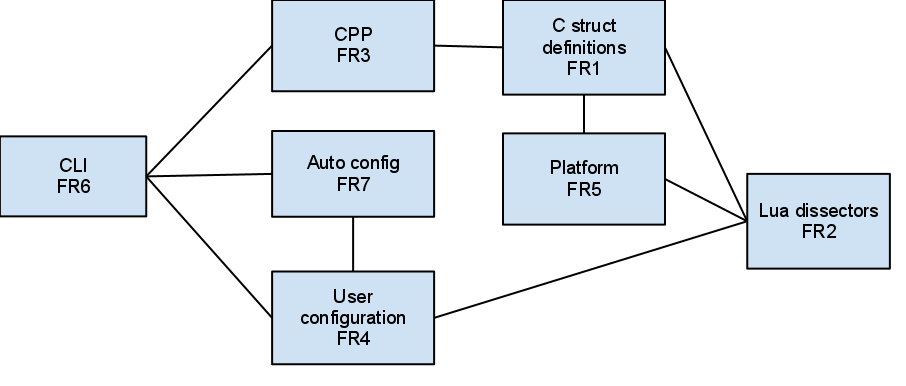
\includegraphics[width=\textwidth]{./planning/img/requirement_relationship}
	\caption{Relationship Between Requirements \label{fig:req:relationship}}
\end{figure}

%------------------
\section{Use Cases}
%------------------
\label{sec:req:usecases}
This sections contains use case diagrams for our two actors, and detailed
textual use cases for these diagrams.

\subsection{Actors}
%------------------
An actor specifies a role played by an external person or thing that interact
with our \gls{utility}. We have three types of actors to consider. First is the
primary actor, that uses the \gls{utility} to generate \glspl{dissector} from 
\Gls{c} header-files. A secondary actor is the user who configures the
\gls{utility} to change the output of it. Finally, we have an offstage actor, which
does not use our \gls{utility} himself, but uses the outputted \glspl{dissector} in \Gls{wireshark}.

We have defined two use case actors for our \gls{utility}. The customer has specified
that the offstage actor, called developer, is the most important actor.
\begin{description}
	\item[Developer] User of the generated \Gls{wireshark} \glspl{dissector}, offstage actor
	\item[Administrator] User and configurer of \gls{utility}, primary and secondary actor
\end{description}

\subsection{Use Case Diagrams}
%-----------------------------
\hyperref[fig:req:ucadm]{Figure \ref*{fig:req:ucadm}} shows the use case
diagram for the administrator, and \autoref{fig:req:ucdev} is the use case
diagram for the developer.
\begin{figure}[htbp]
	\center
	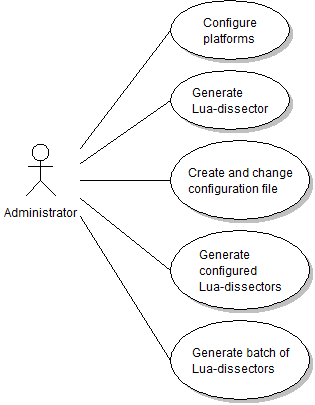
\includegraphics[width=0.6\textwidth]{./planning/img/uc_administrator}
	\caption{Use Case Diagram: Administrator\label{fig:req:ucadm}}
\end{figure}

\begin{figure}[htbp]
	\center
	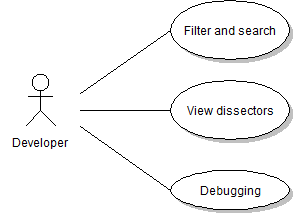
\includegraphics[width=0.6\textwidth]{./planning/img/uc_developer}
	\caption{Use Case Diagram: Developer\label{fig:req:ucdev}}
\end{figure}

\subsection{Textual Use Cases}
%-----------------------------
Here each of the use cases are described textually.

\begin{table}[htbp] \footnotesize \center
\caption{Filter and search textual use case\label{tab:textual:filterandsearch}}
\noindent\makebox[\textwidth]{%
\begin{tabularx}{1.2\textwidth}{l X}
	\toprule
	 & 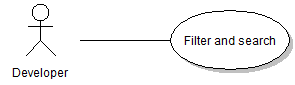
\includegraphics[scale=0.8]{./planning/img/uc_filterandsearch} \\
	\toprule
	Element & Description\\
	\midrule
	Use case name & Filter and search on attributes\\
	Goal & The developer wants the correct set of results based on the search phrase \\
	Summary & The developer would like to filter and search on attributes in the packets displayed in Wireshark \\
	Preconditions & Wireshark need to be running with dissectors. \\
	Postconditions & Wireshark display the results.\\
	\midrule
	\multirow{3}{*}{Flow of Events} & 1. The developer selects the search field in Wireshark's GUI.  \\
	& 2. The user types in a search phrase. \\
	& 3. Wireshark will present the search results that match the query. \\
	\midrule
	Exceptions & None. \\
	\bottomrule
\end{tabularx}}
\end{table}

\begin{table}[htbp] \footnotesize \center
\caption{View dissector textual use case\label{tab:textual:viewdissector}}
\noindent\makebox[\textwidth]{%
\begin{tabularx}{1.2\textwidth}{l X}
	\toprule
	 & 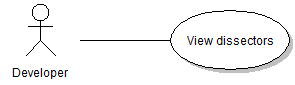
\includegraphics[scale=0.8]{./planning/img/uc_viewdissectors} \\
	\toprule
	Element & Description\\
	\midrule
	Use case name & View the dissectors in Wireshark\\
	Goal & View structs correctly dissected in Wireshark\\
	Summary & The developer would like to dissect a structs and have the members and values displayed in Wireshark by using the dissectors in Wireshakrs plugin folder.\\
	\multirow{2}{*}{Preconditions}& 1. The developer have Wireshark running with dissectors. \\
	& 2. The dissector for a struct will dissect it correctly, according to the initial internal structure of the struct. \\
	Postconditions & Wireshark display the struct with the correct structure and values.\\
	\midrule
	\multirow{3}{*}{Flow of Events} & 1. The developer selects a struct message in Wireshark. \\
	& 2. Wireshark calls the correct dissector and dissects the selected message. \\
	& 3. Wireshark displays the members and values of the selected message. \\
	\midrule
	\multirow{2}{*}{Exceptions} & 1. The correct dissector for a struct might not exist in Wiresharks plugin folder, making it impossible to dissect the message. \\
	& 2. more? \\
	\bottomrule
\end{tabularx}}
\end{table}

\begin{table}[htbp] \footnotesize \center
\caption{Debugging textual use case\label{tab:textual:debugging}}
\noindent\makebox[\textwidth]{%
\begin{tabularx}{1.2\textwidth}{l X}
	\toprule
	 & 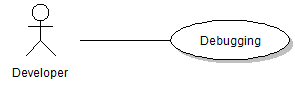
\includegraphics[scale=0.8]{./planning/img/uc_debugging} \\
	\toprule
	Element & Description\\
	\midrule
	Use case name & Filter and search on attributes\\
	Goal & The user wants the correct set of results based on the search phrase \\
	Summary & The user would like to filter and search on attributes in the packets displayed in Wireshark \\
	Preconditions & The user have Wireshark running with dissectors. \\
	Postconditions & Wireshark display the results.\\
	Flow of Events & The user selects the search field in Wireshark's API and types in a search phrase, then Wireshark will present the search results that match the query. \\
	Exceptions & N/A \\
	\bottomrule
\end{tabularx}}
\end{table}

\begin{table}[htbp] \footnotesize \center
\caption{Configure platforms textual use case\label{tab:textual:configureplatforms}}
\noindent\makebox[\textwidth]{%
\begin{tabularx}{1.2\textwidth}{l X}
	\toprule
	 & 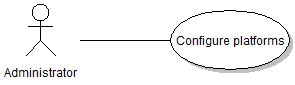
\includegraphics[scale=0.8]{./planning/img/uc_configureplatform} \\
	\toprule
	Element & Description\\
	\midrule
	Use case name & Filter and search on attributes\\
	Goal & The administrator would like to filter and search on attributes in the packets displayed in Wireshark \\
	Summary & \\
	Preconditions & The user have Wireshark running with dissectors. \\
	Postconditions & Wireshark display the results.\\
	Flow of Events & The user selects the search field in Wireshark's API and types in a search phrase, then Wireshark will present the search results that match the query. \\
	Exceptions & N/A \\
	\bottomrule
\end{tabularx}}
\end{table}

\begin{table}[htbp] \footnotesize \center
\caption{Generate Lua dissector textual use case\label{tab:textual:generatelua}}
\noindent\makebox[\textwidth]{%
\begin{tabularx}{1.2\textwidth}{l X}
	\toprule
	 & 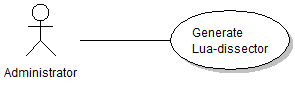
\includegraphics[scale=0.8]{./planning/img/uc_generatelua} \\
	\toprule
	Element & Description\\
	\midrule
	Use case name & Filter and search on attributes\\
	Goal & The user would like to filter and search on attributes in the packets displayed in Wireshark \\
	Summary & \\
	Preconditions & The user have Wireshark running with dissectors. \\
	Postconditions & Wireshark display the results.\\
	Flow of Events & The user selects the search field in Wireshark's API and types in a search phrase, then Wireshark will present the search results that match the query. \\
	Exceptions & N/A \\
	\bottomrule
\end{tabularx}}
\end{table}

\begin{table}[htbp] \footnotesize \center
\caption{Create and change configuration file textual use case\label{tab:textual:configure}}
\noindent\makebox[\textwidth]{%
\begin{tabularx}{1.2\textwidth}{l X}
	\toprule
	 & 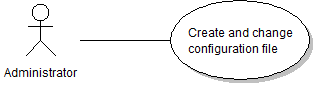
\includegraphics[scale=0.8]{./planning/img/uc_configurate} \\
	\toprule
	Element & Description\\
	\midrule
	Use case name & Filter and search on attributes\\
	Goal & The user would like to filter and search on attributes in the packets displayed in Wireshark \\
	Summary & \\
	Preconditions & The user have Wireshark running with dissectors. \\
	Postconditions & Wireshark display the results.\\
	Flow of Events & The user selects the search field in Wireshark's API and types in a search phrase, then Wireshark will present the search results that match the query. \\
	Exceptions & N/A \\
	\bottomrule
\end{tabularx}}
\end{table}

\begin{table}[htbp] \footnotesize \center
\caption{Generate configured Lua-dissectors textual use case\label{tab:textual:generateconfiglua}}
\noindent\makebox[\textwidth]{%
\begin{tabularx}{1.2\textwidth}{l X}
	\toprule
	 & 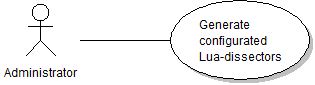
\includegraphics[scale=0.8]{./planning/img/uc_generateconfiglua} \\
	\toprule
	Element & Description\\
	\midrule
	Use case name & Filter and search on attributes\\
	Goal & The user would like to filter and search on attributes in the packets displayed in Wireshark \\
	Summary & \\
	Preconditions & The user have Wireshark running with dissectors. \\
	Postconditions & Wireshark display the results.\\
	Flow of Events & The user selects the search field in Wireshark's API and types in a search phrase, then Wireshark will present the search results that match the query. \\
	Exceptions & N/A \\
	\bottomrule
\end{tabularx}}
\end{table}

\begin{table}[htbp] \footnotesize \center
\caption{Generate batch of Lua dissectors textual use case\label{tab:textual:luabatch}}
\noindent\makebox[\textwidth]{%
\begin{tabularx}{1.2\textwidth}{l X}
	\toprule
	 & 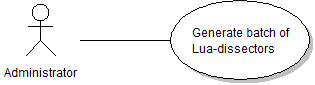
\includegraphics[scale=0.8]{./planning/img/uc_luabatch} \\
	\toprule
	Element & Description\\
	\midrule
	Use case name & Filter and search on attributes\\
	Goal & The user would like to filter and search on attributes in the packets displayed in Wireshark \\
	Summary & \\
	Preconditions & The user have Wireshark running with dissectors. \\
	Postconditions & Wireshark display the results.\\
	Flow of Events & The user selects the search field in Wireshark's API and types in a search phrase, then Wireshark will present the search results that match the query. \\
	Exceptions & N/A \\
	\bottomrule
\end{tabularx}}
\end{table}

\section{User Stories}
To make it easier to implement the requirements, there have been written user stories. The user stories describes how the requirements should be implemented, and was written in each sprint planning meeting. The user stories that are written can be found in the sprint design for each of the sprint. \autoref{tab:us:template} shows an template of an user story.

\begin{table}[htbp] \footnotesize \center
\caption{User Story Template\label{tab:us:template}}
\noindent\makebox[\textwidth]{%
\begin{tabularx}{1.2\textwidth}{l X}
\toprule
Header & Value \\
\midrule
ID & ID for the user stories, written like USxx. \\
Requirements & The requirement that the user story descripbes. \\
What & Description of what the user want to achieve.\\
How & Description of how the requirement should be implemented. \\
Result & What the result is after the implementation. \\
\bottomrule
\end{tabularx}}
\end{table}



\section{Product Backlog}
%------------------------
\label{sec:prodbacklog}
The complete product backlog can be seen in \autoref{tab:prodbacklog}.
Optional requirements which we did not implement are listed in
\autoref{tab:prodbacklog2}. These optional requirements are described
in \autoref{sec:eval:furtherdev}.

\begin{table}[htbp] \small \center
\caption{Optional Requirements Estimates\label{tab:prodbacklog2}}
\begin{tabularx}{\textwidth}{l X c}
	\toprule
	Req. & Description & Est. Hours \\
	\midrule	
	FR2-F & Display if struct member contains uninitialized memory & 8 \\
	FR6-D & Do not regenerate dissectors across multiple runs & 2 \\
	FR7-A & Find struct descriptions from Doxygen comments & 20 \\
	FR7-B & Find configuration of \#define enums from header files & 20 \\
	\midrule
	& Total & 50 \\
	\bottomrule
\end{tabularx}
\end{table}

%\begin{table}[htbp] \footnotesize \center
\begin{table}[htbp] \small \center
\caption{Product Backlog\label{tab:prodbacklog}}
\noindent\makebox[\textwidth]{%
\begin{tabularx}{1.13\textwidth}{l X c c c}
	\toprule
	& & & \multicolumn{2}{c}{Hours} \\
	\cmidrule(r){4-5}
	Req. & Description & Sprint & Est. & Act. \\
	\midrule
	FR1 & Read basic \Gls{c} \gls{struct} definitions & & \textbf{52}  & \textbf{51}  \\
	FR1-A & Support data types: \gls{int}, \gls{float}, \gls{char} and \gls{boolean} & SP1 & 24 & 21 \\
	FR1-B & Support \glspl{member} of type \gls{enum} & SP2 & 6 & 5 \\
	FR1-C & Support \glspl{member} of type \gls{struct} & SP2 & 7 & 3.5 \\
	FR1-D & Support \glspl{member} of type \gls{union} & SP3 & 5 & 6 \\
	FR1-E & Support \glspl{member} of type \gls{array} & SP2 & 7 & 12 \\
	FR1-F & Detect \glspl{struct} with same name & SP2 & 3 & 3.5 \\
	\addlinespace
	FR2 & Generate \Gls{wireshark} \glspl{dissector} in \Gls{lua} & & \textbf{69} &  \textbf{59.5} \\
	FR2-A & Display simple \glspl{struct} & SP1 & 28 & 25 \\
	FR2-B & Support display of \glspl{struct} within \glspl{struct} & SP2 & 11 & 15 \\
	FR2-C & Support \Gls{wireshark} filter and search on attributes & SP3 & 3 & 1.5 \\
	FR2-D & Recognize invalid values for a \gls{struct} \gls{member} & SP1 & 22 & 15 \\
	FR2-E & Guess \glspl{dissector} from packet size & SP4 & 5 & 3\\
    \addlinespace
	FR3 & Support \Gls{c} \gls{preprocessor} directives and macros & & \textbf{24} &  \textbf{7.5}\\
	FR3-A & Support \gls{include} & SP1 & 8 & 2 \\
	FR3-B & Support \gls{define} and \gls{if} & SP1 & 11 & 3 \\
	FR3-C & Support \verb+_WIN32+, \verb+_WIN64+, \verb+__sparc+ etc & SP3 & 5 & 2.5 \\
	\addlinespace
	FR4 & Support user configuration & & \textbf{91} & \textbf{71}\\
	FR4-A & Support valid ranges for \gls{struct} \glspl{member} & SP1 & 30 & 15 \\
	FR4-B & Support custom \Gls{lua} files for specific protocols & SP3 & 10 & 7.5 \\
	FR4-C & Support custom handling of specific data types & SP2 & 6 & 5 \\
	FR4-D & Support specifying the ID of \glspl{dissector} & SP2 & 7 & 9 \\
	FR4-E & Support various \gls{trailers} (other registered protocols) & SP2 & 18 & 15 \\
	FR4-F & Support \glspl{enumerated named value} & SP2 & 5 & 6.5 \\
	FR4-G & Support bit strings & SP2 & 10 & 11.5 \\
	FR4-H & Automatic generation of placeholder configuration & SP4 & 1 & 0.5\\
	FR4-I & Support specifying the size of unknown struct members & SP4 & 4 & 1\\
	\addlinespace
	FR5 & Handle input which size and \gls{endian} depends on platform & & \textbf{40} & \textbf{23.5} \\
	FR5-A & Flags specified for each platform & SP3 & 8 & 11 \\
	FR5-B & \Glspl{dissector} support memory alignment & SP3 & 12 & 6.5 \\
	FR5-C & \Glspl{dissector} support both little and big \gls{endian} & SP3 & 6 & 4 \\
	FR5-D & \Glspl{dissector} support different sizes from flags & SP3 & 14 & 2 \\	
    \addlinespace
	FR6 & Support parameters from command line & & \textbf{51} & \textbf{24}\\
	FR6-A & Support parameter for \Gls{c} \gls{header} file & SP1 & 9 & 9 \\
	FR6-B & Support parameter for configuration file & SP1 & 28 & 8 \\
	FR6-C & Support batch processing of \Gls{c} \gls{header} and configuration & SP2 & 7 & 4.5 \\
	FR6-E & Support C \#defines and --Include from CLI & SP4 & 1 & 1 \\
	FR6-F & Only generate dissectors for structs with valid ID & SP4 & 4 & 1.5 \\
	\midrule
	& Total & & 327 & 236.5 \\
    \bottomrule
\end{tabularx}}
\end{table}	


\end{document}

